\chapter{Preliminaries}
\label{chap:preliminaries}

\section{Basic things}

Following \cite{hesthaven2007nodal}, define orthonormal basis functions $\phi_1, \phi_2, \cdots, \phi_N$ and nodes $\ve r_1, \ve r_1, \cdots, \ve r_N$ on the reference element.

A function $u(\ve r)$ in the space spanned by the basis functions can be uniquely given by its modal coefficients $\hat{u}_1, \cdots, \hat{u}_N$ or by its nodal values $u(\ve r_1), \cdots, u(\ve r_N)$.  The Vandermonde matrix $V_{ij}$ converts modal coefficients to nodal values,
%
\begin{equation}
\boxed{
V = \begin{bmatrix} \phi_1(\ve r_1) & \phi_2(\ve r_1) & \hdots & \phi_N(\ve r_1) \\
\phi_1(\ve r_2) & \phi_2(\ve r_2) & \hdots & \phi_N(\ve r_2) \\
\vdots & \vdots & \ddots & \vdots \\
\phi_1(\ve r_N) & \phi_2(\ve r_N) & \hdots & \phi_N(\ve r_N)
\end{bmatrix}
}
\end{equation}
%
so that $u(\ve r_i) = V_{ij} \hat{u}_j$.

To evaluate a function at non-nodal points we use the Vandermonde matrix and the values of the basis functions at the evaluation points.
%
\begin{equation}
u(r') = \hat{u}_i \phi_i(r') = \ve{u}^T V^{-T} \begin{bmatrix} \phi_1(r') \\ \phi_2(r') \\ \vdots \\ \phi_N(r') \end{bmatrix}.
\label{eqn:interpolation}
\end{equation}

\section{Integration and differentiation on the reference element}

\subsection{Quadrature}

Because the basis functions are orthonormal on the reference element, the Vandermonde matrix can be used for quadrature of functions sampled on nodal points\footnote{Let's go ahead and assume that all functions such as the examples $f(\ve r)$ and $g(\ve r)$ are sums of the basis functions so quadrature is exact.}:
%
\begin{equation}
\int_\bigtriangleup dr \, f(\ve r) g(\ve r) = f(\ve r_i) (V^{-1})_{ji}(V^{-1})_{jk} g(\ve r_k) = \ve f^T V^{-T} V^{-1} \ve g
\end{equation}
%
in various notations.  We define the reference element inner product kernel
%
\begin{equation}
\boxed{
Q = V^{-T} V^{-1}
}
\end{equation}
%
and note that quadrature can be carried out with the kernel $\ve 1^T Q$:
%
\begin{equation}
\int_\bigtriangleup dr \, f(\ve r) = \ve 1^T Q \ve f.
\end{equation}

\subsection{Differentiation}

The gradient of the Vandermonde matrix is calculable from gradients of the basis functions.  The gradient of a function at the nodal points is calculable by decomposing it into basis functions, differentiating them and summing them back up.  Without loss of generality take the derivative in the $r$ direction:
%
\begin{equation}
\boxed{
D_r = \pp{V}{r} V^{-1}
}
\end{equation}
%
\begin{equation}
\renewcommand\arraystretch{1.5}
\begin{bmatrix}
\pp{f}{r}(\ve r_1) \\ \pp{f}{r}(\ve r_2) \\ \vdots \\ \pp{f}{r}(\ve r_N)
\end{bmatrix}
=
D_r \begin{bmatrix} f(\ve r_1) \\ f(\ve r_2) \\ \vdots \\ f(\ve r_N) \end{bmatrix}.
\end{equation}

\section{Coordinate transformations}

Coordinate transformations are ubiquitous in FEM because the elemental equations are all transformed versions of the elemental equations on a single reference element.  For unstructured meshes of triangles or tetrahedra of different sizes and orientations, the governing equations are all ultimately formulated on the reference element.  Curvilinear elements, arising from non-affine coordinate transformations, are particularly gross.

When directly differentiating the FEM system for sensitivity analysis, the sensitivity of the Jacobian plays the central role.  We'll get there too.

\subsection{Transforming the 2D reference element}

Following \cite{hesthaven2007nodal}, take the basis element to be a simplex with vertices $(r,s) = \left\{ (-1,-1), (1,-1), (-1,1) \right\}$ (Fig. \ref{fig:reference_simplex}).
%
\begin{figure}[!ht]
\centerline{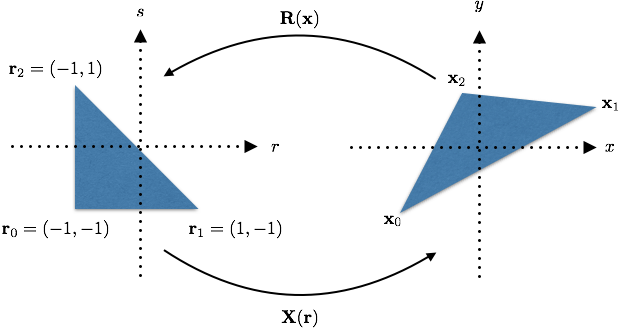
\includegraphics[width=7cm]{reference_simplex.png}}
\caption{The reference simplex (left) and its transformed version (right).  The coordinate transformation $\ve X(\ve r)$ maps $\ve r_0 \mapsto \ve x_0$, $\ve r_1 \mapsto \ve x_1$, and $\ve r_2 \mapsto \ve x_2$.  $\ve{X}(\ve{r})$ and $\ve{R}(\ve{x})$ are inverses of each other.}
\label{fig:reference_simplex}
\end{figure}
%
Points $\ve r = (r,s)$ in the reference simplex are mapped to $\ve x = (x,y)$ in each finite element by the per-element coordinate transformation $\ve X(\ve r; \ve p)$.  The transformation depends on the design parameters $\ve p$ because changing $\ve p$ may change the shapes of structures in the simulation and thus change the mesh.  The mapping $\ve R(\ve x; \ve p)$ is defined as the inverse of $\ve X$, so that for fixed $\ve p$,
%
\begin{equation}
\ve R(\ve X(\ve r; \ve p); \ve p) = \ve r.
\end{equation}
%
Integrals in $(x,y)$ space are performed in $(r,s)$ coordinates to take advantage of the axis-aligned edges of the simplex and the convenient properties of the basis functions.  This necessitates use of the Jacobian, $J(\ve r; \ve p)$,
%
\begin{equation}
\renewcommand\arraystretch{1.5}
J = \nabla_{\ve r} \ve X =
\begin{bmatrix}
\pp{x}{r} & \pp{x}{s} \\
\pp{y}{r} & \pp{y}{s}
\end{bmatrix}.
\end{equation}
%
Most elements are affine, meaning their transformation is of the form\footnote{Due to the choice of reference simplex, this formula is slightly more complicated than would be obtained if $\ve r_0 = (0,0), \ve r_1 = (1,0), \ve r_2 = (0,1)$.}
%
\begin{equation}
\ve X(\ve r) = \frac{\ve x_1 + \ve x_2}{2} + \frac{1}{2}\left(r (\ve x_1 - \ve x_0) + s (\ve x_2 - \ve x_0) \right)
\end{equation}
%
and their Jacobian is
%
\begin{equation}
\renewcommand\arraystretch{1.5}
J =
\begin{bmatrix}
\frac{\ve x_1 - \ve x_0}{2} &  \frac{\ve x_2 - \ve x_0}{2}
\end{bmatrix}.
\end{equation}
This Jacobian is constant over the entire element, which may lead to a simpler implementation of the FEM equations.

\subsection{Inverse parameterized coordinate transform}

Let $\ve X(\ve r; \ve p)$ and $\ve R(\ve x; \ve p)$ be inverses of each other.  
Identify the Jacobian, $J = \D_{\ve r} \ve X$.  We know $\ve X$ analytically and its sensitivity $\ppp{\ve X}{\ve p}$.  What is the sensitivity of the inverse, $\ppp{\ve R}{\ve p}$?

One straightforward approach: define the augmented mappings
%
\begin{equation}
\begin{aligned}
\tilde{\ve X}(\ve r; \ve p) &= \begin{bmatrix} \ve X(\ve r; \ve p) \\ \ve p \end{bmatrix} \\
\tilde{\ve R}(\ve x; \ve p) &= \begin{bmatrix} \ve R(\ve x; \ve p) \\ \ve p \end{bmatrix}
\end{aligned}
\end{equation}
%
which are also each other's inverse.  As inverses, we have that $\D \tilde{\ve X} \cdot \D \tilde{\ve R} = \mathbb{1}$, or
%
\begin{equation}
\begin{bmatrix} \D_{\ve r} \ve X & \D_{\ve p} \ve X \\ \mathbb{0} & \mathbb{1} \end{bmatrix}
\begin{bmatrix} \D_{\ve x} \ve R & \D_{\ve p} \ve R \\ \mathbb{0} & \mathbb{1} \end{bmatrix}
= \mathbb{1}.
\end{equation}
%
This leads directly to the nice answer:
%
\begin{equation}
\label{eqn:inverse_transformation_derivative}
\boxed{
\begin{aligned}
\D_{\ve x} \ve R &= \left( \D_{\ve r} \ve X \right)^{-1} &&= J^{-1}\\
\D_{\ve p} \ve R &= - \left( \D_{\ve r} \ve X \right)^{-1} \D_{\ve p} \ve X &&= -J^{-1} \D_{\ve p} \ve X.
\end{aligned}
}
\end{equation}

\section{Integration and differentiation on transformed elements in $x,y$}

\subsection{Integration}

To carry out inner products on transformed elements, use the Jacobian,
%
\begin{equation}
\int_{\ve X(\bigtriangleup)} dx \, f(\ve x) g(\ve x) = \int_\bigtriangleup dr \, \det \{ J(\ve r) \} f(\ve r) g(\ve r) = f_i Q_{ij} \, (\det \{J\} g)_j.
\end{equation}
%
We might also define a quadrature kernel for transformed elements,
%
\begin{equation}
\boxed{
Q^{(x)} = Q
\begin{bmatrix}
\det J(\ve r_1) & & & \\
& \det J(\ve r_2) & & \\
& & \ddots & \\
& & & \det J(\ve r_N)
\end{bmatrix}.
}
\label{eqn:quadrature_transformed}
\end{equation}
%
In the following, the notation $\operatorname{diag} |J|$ will refer to the matrix in the right hand side of Eqn. \ref{eqn:quadrature_transformed}.

For affine elements, because $\det J$ is a constant, the transformed quadrature matrix is simply $Q^{(x)} = Q \det J$.

\subsection{Differentiation}
By the chain rule, $\nabla_{\ve r} f = \nabla_{\ve x}f J$, so $\nabla_{\ve x}f = \nabla_{\ve r} f J^{-1}$.  To extend to differentiation matrices with general element transformations, let us write out the matrix elements of these expressions more explicitly starting with the inverse Jacobian.
%
\begin{equation}
J^{-1} = \begin{bmatrix}
k_{11} & k_{12} & \hdots \\
k_{21} & k_{22} & \hdots \\
\vdots & \vdots & \ddots
\end{bmatrix}.
\end{equation}
%
In two dimensions, $\nabla_{\ve x} g$ at single nodal points $\ve x_i$ is
%
\begin{equation}
\begin{aligned}
\partial_x g(\ve x_i) = k_{11}(\ve r_i) \partial_r g(\ve x_i) + k_{21}(\ve r_i) \partial_s g(\ve x_i) \\
\partial_y g(\ve x_i) = k_{12}(\ve r_i) \partial_r g(\ve x_i) + k_{22}(\ve r_i) \partial_s g(\ve x_i)
\end{aligned}
\end{equation}
%
where the repeated $i$ index does not imply summation.  The gradients of $\ve g$ at nodes $\ve r_i$ are calculated using the differentiation matrices for the reference element.  The elements of the Jacobian at each point can be handled with diagonal matrices to arrive at expressions for $D_x$ and $D_y$ on the transformed elements:
%
\begin{equation}
\boxed{
\begin{aligned}
D_x &= \mathrm{diag}(\ve k_{11}) D_r + \mathrm{diag}(\ve k_{21}) D_s \\
D_y &= \mathrm{diag}(\ve k_{12}) D_r + \mathrm{diag}(\ve k_{22}) D_s .
\end{aligned}
}
\label{eqn:partialDerivatives}
\end{equation}


\section{Sensitivity of functions and functionals}

Under perturbation of system parameters including the mesh, what happens to the values of functions at the (moving) node positions?  What happens to the values of functions evaluated at fixed points in space?  What happens to evaluation of functionals?

Shape changes in the domain $\Omega$ lead fo changes in triangles $\bigtriangleup$ which express as changes in $J$ when discretizing differential equations.  So we will find certain sensitivities with respect to elements of $J$.

\subsection{Sensitivity of the Jacobian}

Every element has its own analytical expression for $J(\ve r; \ve p)$ and can be differentiated to get $\ppp{J}{\ve p}$.  At times we will need the sensitivity of $J^{-1}$ as well,
%
\begin{equation}
\boxed{
\pp{}{p} J^{-1} = - J^{-1} \pp{J}{p} J^{-1}.
}
\end{equation}
%
Its sensitivity to changes in single elements of $J$ is
%
\begin{equation}
\label{eqn:jacobian_jacobian_sensitivity}
\begin{aligned}
\pp{J^{-1}_{\alpha \delta}}{J_{ij}} &= -J^{-1}_{\alpha \beta} \pp{J_{\beta \gamma}}{J_{ij}} J^{-1}_{\gamma \delta} \\
&= -J^{-1}_{\alpha \beta} \delta_{i \beta} \delta_{j \gamma} J^{-1}_{\gamma \delta} \\
&= -J^{-1}_{\alpha i} J^{-1}_{j \delta}.
\end{aligned}
\end{equation}

%
Frequently we will also need the sensitivity of the Jacobian's determinant, which is
%
\begin{equation}
\boxed{
\pp{}{p} |J| = |J| \operatorname{Tr} \left( J^{-1} \pp{J}{p} \right).
}
\end{equation}
%
Its sensitivity to changes in single elements of $J$ is
%
\begin{equation}
\begin{aligned}
\pp{|J|}{J_{i j}} &= |J| \delta_{\alpha \gamma} \left(  J^{-1}_{\alpha \beta} \pp{J_{\beta \gamma}}{J_{i j}} \right) \\
&= |J| \delta_{\alpha \gamma} \left( J^{-1}_{\alpha \beta} \delta_{\beta i} \delta_{\gamma j} \right) \\
&= |J| \delta_{\alpha \gamma} \left( J^{-1}_{\alpha i} \delta_{\gamma j} \right) \\
&= |J| J^{-1}_{ji}.
\end{aligned}
\end{equation}
%
The ``determinant'' of a nonsquare matrix is used in surface and curve integration.  Its sensitivity is
%
\begin{equation}
\begin{aligned}
\pp{\sqrt{| J^T J |}}{J_{ij}} &= \pp{\sqrt{|J^T J|}}{(J^TJ)_{kl}} \pp{(J^TJ)_{kl}}{J_{ij}} \\
&= \frac{1}{2\sqrt{|J^TJ|}} \pp{|J^T J|}{(J^TJ)_{kl}} \left( \delta_{k j} J_{i l} + J_{i k} \delta_{l j} \right) \\
&= \sqrt{|J^TJ|} \left( J (J^T J)^{-1} \right)_{ij}.
\end{aligned}
\end{equation}
%
I did check this numerically for $2 \times 2$ matrices, O skeptic.


\subsection{Sensitivity of Derivative Matrices}

Knowing $\ppp{J^{-1}}{p}$ we can directly get the sensitivities of $D_x$ and $D_y$ by differentiating Equation \ref{eqn:partialDerivatives},
%
\begin{equation}
\boxed{
\begin{aligned}
\pp{D_x}{p} &= \diag \left( \pp{\ve k_{11}}{p} \right) D_r + \diag \left( \pp{\ve k_{21}}{p} \right) D_s \\
\pp{D_y}{p} &= \diag \left( \pp{\ve k_{12}}{p} \right) D_r + \diag \left( \pp{\ve k_{22}}{p} \right) D_s. \\
\end{aligned}
}
\label{eqn:partialDerivativeSensitivities}
\end{equation}
%
Taking the derivative with respect to elements of the Jacobian,
%
\begin{equation}
\begin{aligned}
\pp{D_x}{J_{ij}} &= \diag \left( -J^{-1}_{1i} J^{-1}_{j1} \right) D_r + \diag \left( -J^{-1}_{2i} J^{-1}_{j1} \right) D_s \\
\pp{D_y}{J_{ij}} &= \diag \left( -J^{-1}_{1i} J^{-1}_{j2} \right) D_r + \diag \left( -J^{-1}_{2i} J^{-1}_{j2} \right) D_s.
\end{aligned}
\end{equation}
%
Again the ``$\diag$'' indicates that the Jacobian sensitivities are to be evaluated node-by-node.

\subsection{Functions}

Let $f(\ve x)$ be defined for all $(x,y)$.  Its values at nodes $x_i$ are the vector $\ve f$ with $f_i = f(\ve{x}_i)$.  As the $\ve{x}_i$ move under mesh perturbation, $\ve f$ will change as
%
\begin{equation}
\boxed{
\dd{}{p} \ve f = \nabla_{\ve x} f \cdot \pp{}{p} \ve X(\ve{r}_i) + \pp{f}{p}.
}
\end{equation}
%
When evaluating $f$ at a non-nodal point $\ve x'$ we use interpolation (Equation \ref{eqn:interpolation}).
%
\begin{equation}
\dd{}{p} u(\ve R(\ve x'))) = \pp{\ve u}{p}^T V^{-T} \phi(\ve R(\ve x')) + \ve{u}^T V^{-T} \left( \nabla_R \phi \cdot \nabla_x \ve R(\ve x') \cdot \pp{\ve x'}{p} \right).
\end{equation}

Let $\phi(\ve r)$ be defined for points $(r,s)$ in the reference element.  (This case probably only occurs with basis elements $\phi$.)  It has been evaluated at an arbitrary point $\ve x$ (not necessarily a node).  Its value at $\ve x$ changes with $p$ because its interpolation from nodal values changes when the nodes shift:
%
\begin{equation}
\boxed{
\dd{}{p} \phi(\ve R(\ve{x})) = \nabla_{\ve r} \phi \cdot \pp{}{p} \ve R(\ve x) = -\nabla_{\ve r} \phi \cdot J^{-1} \pp{}{p} \ve X.
}
\end{equation}

\subsection{Functionals}

A common functional is the inner product of the field solution $u$ against a function $a$.
%
\begin{equation}
I = \int_\bigtriangleup dx \, a u.
\end{equation}
%
We will want its sensitivity
%
\begin{equation}
\begin{aligned}
\dd{I}{p} &= \dd{}{p} \ve{a}^T Q \operatorname{diag} |J| \ve u \\
&= \dd{\ve{a}^T}{p} Q \operatorname{diag} |J| \ve u +
\ve{a}^T Q \dd{\, \operatorname{diag} |J|}{p} \ve u +
\ve{a}^T Q \operatorname{diag} |J| \dd{\ve u}{p}.
\end{aligned}
\label{eqn:discreteFunctionalSensitivity}
\end{equation}
%
The first two terms are\footnote{Need to define better notation than $\ve x$ and $\ve y$ for the node coordinates!!}
%
\begin{equation}
\begin{aligned}
% First term
\dd{\ve{a}^T}{p} Q \operatorname{diag}|J| \ve u &=
%\left( \ve{a}^T D_x^T \diag \partial_p \ve x + \ve{a}^T D_y^T \diag \partial_p \ve y + \partial_p \ve a^T \right) Q |J| \ve u \\
\left( D_x \ve{a} \diag \partial_p \ve x + D_y \ve{a} \diag \partial_p \ve y + \partial_p \ve a \right)^T Q |J| \ve u \\
% Second term
\ve{a}^T Q \dd{\, \diag |J|}{p} \ve u &= \ve {a}^T Q \diag \left\{ |J| \Tr \left( J^{-1} \dd{J}{p} \right) \right\} \ve u.
\end{aligned}
\end{equation}
%
Some things can be grouped together.  :-)





\section{Differential volume for surface integrals}

The change of variables for volume integrals in $\mathbb{R}^n$ is
%
\begin{equation}
\int_\Omega d^n x \, f(\ve x) = \int_{\ve R (\Omega)} d^n r \det \{ J(\ve r) \} f(\ve X (\ve r)).
\end{equation}
%
with a Jacobian $J \in \mathbb{R}^{n \times n}$.  When integrating on an $m$-dimensional surface $\Gamma$ embedded in $\mathbb{R}^n$, the appropriate formula is
%
\begin{equation}
\int_\Gamma d^m x \, f(\ve x) = \int_{\ve R(\Gamma)} d^m r \, \sqrt{\det \{ J^T J \} }\,  f(\ve X(\ve r))
\label{eqn:surface_integral}
\end{equation}
%
where $\ve r \in \mathbb R^m$, but still $\ve x \in \mathbb R^n$.  Here I explain the origin of the strange area term $\sqrt{ \det \{J^T J \} }$.  Because $J \in \mathbb{R^{n \times m}}$ is not square, its determinant is undefined and we must seek another method to find the differential area.  In fact this is quite simple.  The columns of the Jacobian are $m$ vectors in $\mathbb R^n$:
%
\begin{equation}
\renewcommand\arraystretch{1.5}
J = 
\begin{bmatrix}
\pp{\ve x}{r_1} & \pp{\ve x}{r_2} & \cdots & \pp{\ve x}{r_m}
\end{bmatrix}.
\end{equation}
%
These columns span an $m$-dimensional parallelepiped $P^m$ embedded in $\mathbb R^n$ and we seek a formula for its ``area''.  Append to these columns orthonormal vectors $\ve u_{m+1}, \cdots, \ve u_n$ which are linearly independent of all the columns of $J$, to give a square matrix $A \in \mathbb R^{n \times n}$,
%
\begin{equation}
\renewcommand\arraystretch{1.5}
A = 
\begin{bmatrix}
\pp{\ve x}{r_1} & \pp{\ve x}{r_2} & \cdots & \pp{\ve x}{r_m} &
\ve u_{m+1} & \cdots & \ve u_{n}
\end{bmatrix}.
\end{equation}
%
Its columns span an $n$-dimensional parallelepiped $P^n$ with volume $\det \{ A \}$.  Because $P^n$ was formed by extruding $P^m$ perpendicularly by a distance of 1 along directions $\ve u_{m+1}$ \emph{etc.}, we have that
%
\begin{equation}
\mathrm{volume} \, P^n = \mathrm{area} \, P^m.
\end{equation}
%
This is the differential area we want for our integral.  In principle once we calculate the extra unit vectors $\{\ve u_i\}$ we can use $\det \{ A \}$, but appending the orthogonal vectors is a bit clumsy and tedious.  Note however the following:
%
\begin{equation}
\begin{aligned}
\renewcommand\arraystretch{1.5}
\det \{A^T \} &= \det \{ A \} \\
\det \{A^T A \} &= \det \{ A \} ^2 \\
A^T A &=
\begin{bmatrix}
(\pp{\ve x}{r_1})^T \\
(\pp{\ve x}{r_2})^T \\
\cdots \\
(\pp{\ve x}{r_m})^T \\
\ve u_{m+1}^T \\
\cdots \\
\ve u_n^T
\end{bmatrix}
\begin{bmatrix}
\pp{\ve x}{r_1} &
\pp{\ve x}{r_2} &
\cdots &
\pp{\ve x}{r_m} &
\ve u_{m+1} &
\cdots &
\ve u_n
\end{bmatrix}
=
\begin{bmatrix}
J^T J & 0 \\ 0 & \mathbb{1}
\end{bmatrix} \\
\therefore \det \{ A^T A \} &= \det \{ J^T J \}.
\end{aligned}
\end{equation}
%
The extra orthogonal vectors are eliminated, leaving a tidy formula.  So the volume of $P^m$ is $\sqrt{ \det \{ J^T J \} }$ and Eqn. \ref{eqn:surface_integral} is justified---at least by physicist standards.

\section{Poisson equation in weak form}

To build a simple electrostatic FEM code let's put the Poisson equation into weak form!
%
\begin{equation}
\begin{aligned}
\partial_i^2 \phi &= f \qquad &&\textrm{on $\Omega$} \\
\phi &= \phi_d \qquad &&\textrm{on $\partial \Omega^d$} \\
\partial_n \phi &= e_n \qquad &&\textrm{on $\partial \Omega^n$.}
\end{aligned}
\end{equation}
%
Because I am a simpleton and cannot figure out how to write down an FEM system for places where Dirichlet boundaries abut Neumann boundaries or where multiple materials join at one point, all these cases are excluded.  Let's imagine that the outer boundary of the system is a Neumann boundary and electrodes (Dirichlet boundaries) are floating around the inside.

To derive the weak form, integrate against a test function $\psi$,
%
\begin{equation}
\int_\Omega \psi \partial_i^2 \phi = \int_\Omega \psi f
\end{equation}
%
and integrate by parts,
%
\begin{equation}
\oint_{\partial \Omega} \psi \partial_n \phi - \int_\Omega (\partial_i \psi)(\partial_i \phi) = \int_\Omega \psi f.
\end{equation}
%
Discretize by meshing $\Omega$ into triangles and representing $\phi$ and $\psi$ as piecewise polynomials with values defined on the nodes in each element.  You know, FEM.  Using the differentiation, quadrature and coordinate transformation operations defined above, turn the weak-form PDE into a linear algebraic expression:
%
\begin{equation}
\begin{aligned}
%&\sum_\textrm{Neumann edges} \psi^T L^T Q^\textrm{1d} |J^\textrm{1d}| L \left( n_x D_x + n_y D_y \right) \phi \\
- &\sum_\bigtriangleup \psi^T \left(D_x^T Q |J| D_x + D_y^T Q |J| D_y \right) \phi \\
= &\sum_\bigtriangleup \psi^T Q |J| f - \sum_\textrm{Neumann edges} \psi^T L^T Q^\textrm{1d} |J^\textrm{1d}|e_n.
\end{aligned}
\end{equation}
%
The $L$ matrix randomly introduced here is the matrix responsible for selecting the nodes of a given edge.  Because on Neumann edges we have fixed the value of $\partial_n \phi = e_n$, the Neumann terms end up on the right-hand side.  I sure hope I am doing this right!!

We will require this equation to hold for all test functions $\psi$.  As test functions we select Lagrange polynomials for each non-Dirichlet node in the system.  The sum over edges only exists when a Neumann boundary is present in the system.  We solve for the values of $\phi$ at all non-Dirichlet nodes in the system.  It boils down to $Ax = b$:
%
\begin{equation}
- \sum_\bigtriangleup (D_x^T Q |J| D_x + D_y^T Q |J| D_y)
\phi
=
\sum_\bigtriangleup Q |J| f + \sum_\textrm{Neumann edges} L^T Q^\textrm{1d} |J^\textrm{1d}|e_n.
\end{equation}
